\documentclass{article}

% if you need to pass options to natbib, use, e.g..
\PassOptionsToPackage{numbers, compress}{natbib}
% before loading neurips_2026

% The authors should use one of these tracks.
% Before accepting by the NeurIPS conference, select one of the options below.
% === SIMBIOCHEM II (NeurIPS 2026 workshop) ===
% SIMBIOCHEM II is a double-blind, non-archival workshop. Use this for submission.
\usepackage[dblblindworkshop]{neurips_2026}
% line numbers are a submission convention; enabled by default for review (kept per user preference)
% For the camera-ready (accepted) version, switch to.
%   \usepackage[dblblindworkshop, final]{neurips_2026}
% This sets the footer, which on the camera-ready reads.
%   "Accepted as a Workshop Paper at the 2nd SIMBIOCHEM, NeurIPS 2026."
\workshoptitle{2nd SIMBIOCHEM Workshop at NeurIPS 2026}
% ---
% the "default" option is equal to the "main" option, which is used for the Main Track with double-blind reviewing.
% 1. "main" option is used for the Main Track
%  \usepackage[main]{neurips_2026}
% 2. "position" option is used for the Position Paper Track
%  \usepackage[position]{neurips_2026}
% 3. "eandd" option is used for the Evaluations & Datasets Track
 % \usepackage[eandd]{neurips_2026}
% 4. "creativeai" option is used for the Creative AI Track
%  \usepackage[creativeai]{neurips_2026}
% 5. "sglblindworkshop" option is used for the Workshop with single-blind reviewing
 % \usepackage[sglblindworkshop]{neurips_2026}
% 6. "dblblindworkshop" option is used for the Workshop with double-blind reviewing
%  \usepackage[dblblindworkshop]{neurips_2026}
% 7. "education" option is used for the Education Track
%  \usepackage[education]{neurips_2026}

% After being accepted, the authors should add "final" behind the track to compile a camera-ready version.
% 1. Main Track
 % \usepackage[main, final]{neurips_2026}
% 2. Position Paper Track
%  \usepackage[position, final]{neurips_2026}
% 3. Evaluations & Datasets Track
 % \usepackage[eandd, final]{neurips_2026}
% 4. Creative AI Track
%  \usepackage[creativeai, final]{neurips_2026}
% 5. Workshop with single-blind reviewing
%  \usepackage[sglblindworkshop, final]{neurips_2026}
% 6. Workshop with double-blind reviewing
%  \usepackage[dblblindworkshop, final]{neurips_2026}
% Note. For the workshop paper template, both \title{} and \workshoptitle{} are required, with the former indicating the paper title shown in the title and the latter indicating the workshop title displayed in the footnote.
% For workshops (5., 6.), the authors should add the name of the workshop, "\workshoptitle" command is used to set the workshop title.
% \workshoptitle{WORKSHOP TITLE}
% 7. Education Track
% \usepackage[education, final]{neurips_2026}

% "preprint" option is used for arXiv or other preprint submissions
 % \usepackage[preprint]{neurips_2026}

% to avoid loading the natbib package, add option nonatbib.
%    \usepackage[nonatbib]{neurips_2026}

\usepackage[utf8]{inputenc} % allow utf-8 input
\usepackage[T1]{fontenc}    % use 8-bit T1 fonts
\usepackage{hyperref}       % hyperlinks
\hypersetup{pdfauthor={}}   % keep PDF metadata anonymous under double-blind review
\usepackage{url}            % simple URL typesetting
\usepackage{booktabs}       % professional-quality tables
\usepackage{amsfonts}       % blackboard math symbols
\usepackage{amsmath}        % \text{} inside math (needed by our math notation)
\usepackage{nicefrac}       % compact symbols for 1/2, etc.
\usepackage{microtype}      % microtypography
\usepackage{xcolor}         % colors
\usepackage{graphicx}       % figures
\usepackage{times}
% Note. For the workshop paper template, both \title{} and \workshoptitle{} are required, with the former indicating the paper title shown in the title and the latter indicating the workshop title displayed in the footnote.
\title{Shrinkage Needs a Gauge: Identifiability and Test-Time Correction of Additive Molecular Energy Predictions}

% The \author macro works with any number of authors. There are two commands
% used to separate the names and addresses of multiple authors. \And and \AND.
%
% Using \And between authors leaves it to LaTeX to determine where to break the
% lines. Using \AND forces a line break at that point. So, if LaTeX puts 3 of 4
% authors names on the first line, and the last on the second line, try using
% \AND instead of \And before the third author name.

% Author block. real author info (source-only; not rendered under
% dblblindworkshop without final/preprint). Anonymity for the review copy is
% handled by the style file; PDF metadata is suppressed via \hypersetup above.



\begin{document}

\maketitle

\begin{abstract}
  Graph Neural Networks have been able to predict molecular properties, such as hydration free energy, with high average accuracy almost from the beginning, but knowing when a prediction is wrong for a specific molecule remains an open problem. The standard approach, ensemble disagreement, misses a systematic class of failures: molecules where the ensemble members agree with each other yet are still far from the true value. We propose correcting these failures directly, by shrinking each atom's predicted contribution toward a population mean at test time, weighted by ensemble uncertainty. This has a basic identifiability problem: a molecule's total predicted property is well-defined, but its decomposition into atomic contributions is not, so two decompositions can agree on every observable quantity and still imply different corrections. We introduce Gauge-Invariant Molecular Shrinkage (GIMS), which resolves this by aggregating atom-level reliability into a one correction strength per molecule, making the result provably invariant to this ambiguity. Despite discarding atom-level detail, GIMS matches or exceeds a variance-weighted atomic baseline and significantly outperforms a strength-matched uniform baseline. We also show that the correction does not transfer as-is to an out-of-domain test set, but a lightweight recalibration recovers a consistent gain, suggesting the approach generalizes with modest adaptation.
\end{abstract}
% VERIFIED. 18/129=14\% quadrant split = deep_ensemble/rmse_analysis/analyze_std_vs_rmse.py; ext. MAE 1.475 R2 0.854 = verification/expdb_external/results/expdb_conformers.hdf5 run; GIMS vs uniform significant on 4/5 (see Results); Gauge VW 3.26 vs GIMS 2.49e-14 = node_refinement/Gauge_invariant_shrinkage/gims_report.json:Gauge_stress and Gauge_INVARIANT_SHRINKAGE_RESULTS.md.

\section{Introduction}
\label{sec:intro}

Hydration free energy, the energy of moving a molecule from vacuum into
water, is central to drug discovery~\cite{mobley2014freesolv}. Graph Neural Networks have predicted it to within an error of a few tenths of a kcal/mol on FreeSolv almost since their introduction~\cite{zhang2022}, but average accuracy is not enough: a model
right on average can still be confidently wrong on a specific molecule.

The standard fix is ensemble disagreement -- training several models that
differ only in seed and using their spread as an uncertainty signal. On
FreeSolv, this fails in the worst way possible: many molecules have close
ensemble agreement while still far from the true value, and this is not
explained by structural isolation, feature density, or interaction cutoff.

Rather than detect these failures, we correct them. DimeNet++ predicts
energy as a sum of per-atom contributions, so a natural fix is to shrink
each atom toward a pool mean, weighted by ensemble disagreement. This
rests on a false premise: a molecule's total energy is well-defined, but
that total energy's split across atoms is not, so two decompositions can agree on
everything observable and still imply different corrections.

We introduce Gauge-Invariant Molecular Shrinkage (GIMS), which averages
atom-level reliability into one strength per molecule before correcting
the total -- invariant to how the model splits energy internally, and
more effective than atom-level or uniform correction. Any architecture
predicting energy as a sum over atoms (DimeNet, SchNet, PaiNN, NequIP,
MACE) shares this ambiguity. We also test whether the correction transfers to an external, out-of-domain set of molecules: the flat correction does not transfer as-is, but a simple recalibration of it does.


\begin{figure}[t]
  \centering
  \includegraphics[width=1\columnwidth]{figure1.png}
  \caption{\textbf{0}, Five seeds on the same molecule give slightly different per-atom predictions. \textbf{1}, Hydration free energy is the energy change when a molecule moves from gas into water. \textbf{2}, For many molecules, the ensemble agrees but is the prediction is still wrong. \textbf{3}, Darker atoms mean the ensemble disagrees more and need more correction. \textbf{4}, The same molecule can have different valid atomic splits with identical total energy. \textbf{5a}, VW shrinks each atom then sums, the two splits give different results. \textbf{5b}, GIMS averages reliability to one strength then shrinks once, the two splits give the same result. \textbf{6}, GIMS beats uniform on most cases, the flat prior fails on new data, and composition-aware correction rescues the worst cases.}
  \label{fig:gims-overview}
\end{figure}


\section{Method}
\label{sec:method}

\subsection{Ensemble Uncertainty and Atom-Level Shrinkage}

For molecule $m$ and ensemble member $k$, let $P_{mi}^{(k)}$ denote the contribution of an atom $i$, with molecular prediction:
\begin{equation}
    E_m^{(k)} = \sum_{i=1}^{N_m} P_{mi}^{(k)} 
\end{equation}
where $N_m$ denotes the number of atoms in molecule $m$. 
Given an ensemble of $K$ models, we compute the mean and sample variance of each atomic contribution across ensemble members:
\[
\bar{P}_{mi}=\frac{1}{K}\sum_{k=1}^{K}P_{mi}^{(k)},
\qquad
\sigma_{mi}^2=\frac{1}{K-1}\sum_{k=1}^{K}\left(P_{mi}^{(k)}-\bar{P}_{mi}\right)^2.
\]


\paragraph{Confidently Wrong Molecules} For each test molecule, we quantify ensemble uncertainty using the cross-member standard deviation of the molecular predictions, $\hat{\sigma}_m$, and prediction error using RMSE against the experimental target. We define confidently wrong molecules as those with below-median ensemble spread and above-median prediction error.

% VERIFIED. cutoff-radius null = node_refinement/cutoff_bias_check/cutoff_bias_check.py on 129 test mols ($|$rho$| < 0.07$ vs n\_heavy/diameter/Rg/frac6A, within-tercile $p > 0.2$; wrong-18/gradient-12 MWU $p > 0.06$, medians smaller); docs/progress/CUTOFF_BIAS_CHECK_RESULTS.md.
% VERIFIED. quadrant split = deep_ensemble/rmse_analysis/analyze_std_vs_rmse.py on aggregate/per_molecule.csv (ensemble_std == std across the 5 per-molecule seed preds, max diff 4.9e-7); 18/129 = 13.95%.
% VERIFIED. disagree33 = top quartile (33/129) of the three-seed per-molecule ensemble std std3 = t[[pred_seed42, pred_seed123, pred_seed999]].std(axis=1, ddof=1), build_populations() in deep_ensemble/repair_data/test_time_repair.py:107-121 (replicated v1_verify.py:100-113); NOT gated-atom-based (the node gate is separate, 2,904/11,613 atoms).

\paragraph{Atom-Level Shrinkage}
We first consider a direct atom-level correction that shrinks each atomic contribution toward a reference mean. For ensemble member $k$,
\begin{equation}\label{eq:atom_shrink}
    \hat{P}_{mi}^{(k)}
=(1-\lambda_{mi})P_{mi}^{(k)}+\lambda_{mi}\mu_T^{(k)},
\end{equation}
where $\lambda_{mi}\in[0,1]$ controls the shrinkage strength and $\mu_T^{(k)}$ is the mean atomic contribution computed over all atoms in the training set. The corrected molecular prediction for ensemble member $k$ and the final ensemble prediction are given by
$$
\hat{E}_{m}^{(k)}=\sum_{i=1}^{N_m}\hat{P}_{mi}^{(k)},\qquad\hat{E}_{m}=\frac{1}{K}\sum_{k=1}^{K}\hat{E}_{m}^{(k)}.
$$
We consider two choices of the shrinkage strength. The uniform baseline applies a constant shrinkage strength $\bar{\lambda}$ to all atoms, whereas\textbf{ variance-weighted (VW)} shrinkage assigns
$$
\lambda_{mi}
=
\frac{\sigma_{mi}^2}{\sigma_{mi}^2+\tau^2},
$$
where $\tau^2$ is a scale parameter selected on the validation set.
For a controlled comparison, the uniform baseline is strength-matched to VW by setting
$\bar{\lambda}$ to the mean shrinkage strength of the VW estimator.


\subsection{Non-identifiability of Atomic Decomposition}
The molecular prediction is well-defined, but its decomposition into atomic contributions is not unique. Consider a shift $g_{mi}$ that is shared across ensemble members and satisfies
$
\sum_{i =1}^{N_m} g_{mi} = 0
$. Define a new atomic decomposition by
\begin{equation}\label{eq:add_Gauge}
    P_{mi}^{(k)\prime} = P_{mi}^{(k)} + g_{mi}
\end{equation}
Because the shift sums to zero within molecule $m$, the molecular prediction is unchanged. Moreover, since $g_{mi}$ is the same for every ensemble member, the cross-ensemble variance of each atomic contribution is unchanged, and therefore so is the shrinkage weight $\lambda_{mi}$.

Variance-weighted (VW) shrinkage, however, is not invariant to this transformation. Based on Eq.\ref{eq:atom_shrink}, under the shifted decomposition, the corrected molecular prediction changes by
$$
\hat{E}_{m,\mathrm{VW}}^{(k)\prime}
-
\hat{E}_{m,\mathrm{VW}}^{(k)}
=
-
\sum_{i=1}^{N_m} \lambda_{mi} g_{mi}.
$$

Thus, two atomic decompositions can produce the same molecular prediction and the same atom-level uncertainty estimates, yet yield different VW corrections. When the shrinkage weights are not identical across atoms, the magnitude of this difference can be made arbitrarily large by scaling an appropriate zero-sum shift.

Therefore, VW shrinkage depends on the particular atomic decomposition produced by the model, even though that decomposition is not uniquely determined. This motivates a correction that is invariant to such zero-sum re-allocations.


% The same algebra reveals a second, related identity. Let $\Lambda_m =
% \frac{1}{N_m}\sum_i \lambda_{mi}$ denote the molecule-level average of the
% shrinkage weights, and let $\widetilde{E}_{m,\mathrm{GIMS}}^{(k)}$ be the
% molecular correction we introduce in the next section. Then
% \[
% \hat{E}_{m,\mathrm{VW}}^{(k)} - \widetilde{E}_{m,\mathrm{GIMS}}^{(k)}
% = -N_m \operatorname{Cov}_{i=1,\dots,N_m}(\lambda_{mi},P_{mi}^{(k)}) .
% \]
% This covariance -- taken across the atoms of a single molecule $m$ -- is
% not identifiable from data. It depends on the arbitrary alignment between
% where the network happens to place a molecule's energy and where it
% happens to place its uncertainty, and no amount of additional data can
% resolve that alignment without first fixing a Gauge. So two decompositions can agree on everything that's actually observable, and still give different VW corrections — differing by exactly this covariance term.


\subsection{Gauge-Invariant Molecular Shrinkage}
GIMS removes the Gauge dependence of atom-level shrinkage by first aggregating the atom-level shrinkage weights within each molecules. Define
$$
\Lambda_m := \frac{1}{N_m}\sum_{i=1}^{N_m}\lambda_{mi} ,
$$

For each ensemble member $k$, GIMS then applies this single shrinkage
strength directly to the molecular prediction:

$$
\widetilde{E}_m^{(k)}
=
(1-\Lambda_m)E_m^{(k)}
+
\Lambda_m N_m \mu_{\mathcal T}^{(k)}.
$$

The final prediction is obtained by averaging over ensemble members,

$$
\widetilde{E}_m
=
\frac{1}{K}
\sum_{k=1}^{K}
\widetilde{E}_m^{(k)}.
$$

Thus, unlike VW, which shrinks individual atomic contributions before
summing them, GIMS first averages the atom-level shrinkage weights and
then shrinks the molecular prediction once.

GIMS is invariant to the zero-sum re-allocations. Under Eq.\ref{eq:add_Gauge} the molecular prediction $E_m^{(k)}$ and the atom-level shrinkage weights $\lambda_{mi}$ remain unchanged. Therefore $\Lambda_m$ also remains unchanged, and hence
$$
\widetilde{E}_m^{(k)\prime}=\widetilde{E}_m^{(k)}.
$$

The relationship between VW and GIMS can be written explicitly as
\begin{equation}
    \hat{E}_{m,\mathrm{VW}}^{(k)}-\widetilde{E}_m^{(k)}=
-N_m\operatorname{Cov}_{i=1,\dots,N_m}\left(\lambda_{mi},P_{mi}^{(k)}\right)
\end{equation}

Therefore, the difference between the two corrections is exactly a within-molecule covariance between the shrinkage weights and the atomic decomposition. This term is Gauge-dependent: it can change under a zero-sum reallocation of atomic contributions even when the molecular prediction and the shrinkage weights remain unchanged. GIMS removes this Gauge-dependent within-molecule term.

% ============

% GIMS uses the same atom-level signal $\lambda_{mi}$ as VW, but changes the
% order of operations: it aggregates first, and only then shrinks. For each
% molecule, define the molecule-level average shrinkage strength
% \[
% \Lambda_m = \frac{1}{N_m}\sum_{i=1}^{N_m}\lambda_{mi} ,
% \]
% and use it to correct the molecular total directly, for each ensemble
% member $k$:
% \[
% \widetilde{E}_m^{(k)} = (1-\Lambda_m)E_m^{(k)} + \Lambda_m N_m \mu_{\mathcal T}^{(k)},
% \]
% where $\mu_{\mathcal T}^{(k)}$ is the training pool's mean per-atom
% contribution, and the final prediction is the ensemble average
% $\widetilde{E}_m=\frac1K\sum_k\widetilde{E}_m^{(k)}$. In words, GIMS
% shrinks the molecular total toward $N_m\mu_{\mathcal T}^{(k)}$ with a single
% strength $\Lambda_m$, rather than shrinking each atom separately.

% This construction is exactly invariant to the ambiguity described above.
% Recall that a seed-independent, zero-sum shift $g_{mi}$ leaves $\Lambda_m$,
% $E_m^{(k)}$, $N_m$, and $\mu_{\mathcal T}^{(k)}$ all unchanged, since none
% of them depend on how energy is split between individual atoms. It follows
% immediately that
% \[
% \widetilde{E}_m^{(k)\prime}=\widetilde{E}_m^{(k)} ,
% \]
% so GIMS cannot be moved by a shift that leaves every observable quantity
% unchanged. This invariance holds exactly on paper, and we confirm it
% numerically as well: under an atom-RMS 1.0~kcal/mol perturbation aligned
% with $\lambda_{mi}-\Lambda_m$, GIMS shifts by only
% $\sim2.5\times10^{-14}$~kcal/mol, while VW shifts by 3.26~kcal/mol. This matches what our formula predicted
% almost exactly (within $\sim2.5\times10^{-14}$), confirming the derivation
% above is correct.

% The reference mean $\mu_{\mathcal T}$ is computed only from the 411
% fold-0 training molecules (7{,}389 atoms), with no test-set values used at
% all. This is a deliberate choice: it keeps the method inductive, meaning it
% can be applied to new molecules without retraining, and safe to deploy,
% since it never looks at the data it is being evaluated on. We also check a
% pooled version using all 11{,}613 available atoms (Section~\ref{para:ref-reconciliation}), and find the
% two versions differ by at most 0.08~kcal/mol on the full test set --
% confirming this choice does not materially affect the result.



% VERIFIED. disagree33 = top quartile (33/129) of the three-seed per-molecule ensemble std std3 = t[[pred_seed42, pred_seed123, pred_seed999]].std(axis=1, ddof=1), build_populations() in deep_ensemble/repair_data/test_time_repair.py:107-121 (replicated v1_verify.py:100-113); NOT gated-atom-based (the node gate is separate, 2,904/11,613 atoms).
% VERIFIED. atypical33 = top quartile (33/129) of GMM NLL (negative log-likelihood, high = atypical/low density) from GMM on PCA of training latents, and union50 = disagree33 U atypical33 (50 = 33+33-16 overlap), same build_populations() deep_ensemble/repair_data/test_time_repair.py:107-121; all129 and gradient12 are the full 129-molecule test set and its 12-molecule gradient-isolated subset.

\section{Experimental Setup}
\label{sec:setup}

\paragraph{Data} We use experimental hydration free energies for 642 small
molecules from FreeSolv~\cite{mobley2014freesolv}. FreeSolv does not report
per-molecule uncertainties, so we treat all labels as point values. Conformers
are generated with RDKit (ETKDGv3, seed 42, MMFF94-optimized): one conformer
is stored per molecule for training, while at test time we generate five
fresh conformers and average predictions across them (TTA-5),
$\hat{y} = \frac{1}{5}\sum_{c=1}^{5} f(\mathbf{x}^{(c)})$. We apply the same
protocol to the external set described in Section~\ref{sec:external}.

\paragraph{Model} We use a DimeNet++-style architecture, specifically
DimeNetPlusSE with its self-interaction and multi-aggregate components
disabled -- equivalent to plain DimeNet++ -- with 128 hidden units, 3
interaction blocks, 7 spherical and 6 radial Bessel functions, a 6.0~\AA{}
cutoff, 32 neighbors, and envelope exponent 5. Per-atom energy contributions
are enabled, so the molecular prediction is the sum of atomic contributions,
\[
E_{\mathrm{mol}} = \sum_{i=1}^{N_{\mathrm{atoms}}} P_i ,
\]
where $P_i$ is the contribution of atom $i$.

\paragraph{Training}  Training proceeds in three stages. Stage 1 pretrains the
backbone on [N] Aquamarine conformers (59{,}783 conformers across 1{,}653
molecules, PBE0+MBD level of theory) with a force-weighted loss. Stage 2
trains a solvation head on top of the frozen backbone using paired
$\Delta G = E_{\mathrm{sol}} - E_{\mathrm{gas}}$ values (scaled by 23.0605).
Stage 3 fine-tunes the full model on FreeSolv (learning rate $10^{-4}$,
weight decay $10^{-5}$, batch size 8, up to 200 epochs with early stopping
at patience 30).

\paragraph{Uncertainty} To estimate node-level uncertainty, we train a
five-seed ensemble of the fold-0 model (seeds 42, 123, 7, 2024, 999), sharing
Stages 1 and 2 across seeds and varying only the Stage 3 fine-tuning. Our
primary analysis uses the three-seed subset $\{42, 123, 999\}$; the remaining
two seeds show a documented pathology in one conformer regime, discussed in
the Appendix.

\paragraph{Evaluation Protocol} We use a frozen five-fold split: molecules are
sorted by experimental value and assigned to folds round-robin, and each fold
is further divided into train/validation/test (20\% test, then 20\% of the
remainder for validation), giving 411/102/129 molecules in fold 0. We train
and evaluate one model per fold, and report the headline result as test MAE
averaged across all five folds. Fold 0 is verified end-to-end -- its split,
checkpoints, and metrics all reproduce the recorded values -- while folds
1--4 are reported from previously recorded metrics. For an additional
robustness check, we randomly split the fold-0 test set in half, into H1
($n=64$) and H2 ($n=65$). H1 is used to recalibrate method hyperparameters
and H2 is used to score the resulting corrections, so that no correction is
calibrated and evaluated on the same molecules. We test every correction on this 129-molecule fold-0 test set, and on five smaller subsets within it, chosen to check whether the correction helps most where it is needed.

\paragraph{Metrics and Test Populations} We report MAE, RMSE, $R^2$, and Kendall $\tau$, along
with $\Delta$MAE against the raw ensemble mean and 10{,}000-sample
bootstrap 95\% confidence intervals. To see whether corrections help most
where they're needed, we test on five populations of the fold-0 test set.
\emph{disagree33} contains the 33 of the 129 fold-0 test molecules where the three-seed
ensemble disagrees with itself the most, ranked by $\hat\sigma_m$.
\emph{atypical33} contains the 33 molecules that look most atypical to the
model, ranked by negative log-likelihood under a Gaussian mixture model
fit to training-set latents. \emph{union50} is the two combined (50 molecules, of which 16 are flagged by both), and
\emph{all129} is the full test set. \emph{gradient12} is the twelve
confidently-wrong molecules left over after ruling out isolation, feature
density, and interaction cutoff (Section~\ref{sec:intro}). FreeSolv has no
per-molecule uncertainties, so every uncertainty estimate here comes from
the model, not the data.



\section{Results and External Generalization}
\label{sec:external}

\subsection{Baselines and The Recorded Headline}

The fold-0 five-seed ensemble mean achieves a test MAE of 0.5059 kcal/mol
(RMSE 0.7696, $R^2$ 0.9646) on the 129 test molecules. The five-fold
headline is $0.549 \pm 0.024$ kcal/mol (per-fold 0.515/0.537/0.581/0.570/0.540;
pooled RMSE 0.921, $R^2$ 0.9427) and is fully regenerable from archived
per-fold checkpoints. All correction methods below use the three-seed subset
$\{42,123,999\}$ and are scored against the corresponding three-seed
uncorrected mean (Table~\ref{tab:arms} baseline, around 4.8 on all129); the
five-seed headline is a separate, pathology-free overall number. All
intervals are 10{,}000 paired-bootstrap 95\% CIs.

\subsection{Atom-Level Correction is capped}

\begin{table}[htbp]
  \caption{Test-set correction quality, reported as change in MAE
(kcal/mol) relative to the uncorrected ensemble mean. Negative values
indicate improvement. The Baseline row gives uncorrected MAE. 95\% CIs
from 10{,}000 paired bootstrap draws are given in
Appendix~\ref{app:protocol}. Populations are defined in
Section~\ref{sec:setup}.}
  \label{tab:arms}
  \centering
  \renewcommand{\arraystretch}{1.2}
  \setlength{\tabcolsep}{10pt}
  \small
  \begin{tabular}{@{}l@{\hspace{6pt}}ccccc@{}}
    \toprule
    Method & disagree33 & atypical33 & union50 & all129 & gradient12 \\
    \midrule
    Baseline MAE & 10.46 & 10.28 & 8.29 & 4.84 & 2.91 \\
    \midrule
    Trust-weighted & $-3.81$ & $-3.82$ & $-2.36$ & $-0.76$ & $+0.67$ \\
    Uniform (matched) & $-5.87$ & $-5.90$ & $-4.09$ & $-1.76$ & $-0.47$ \\
    Variance-weighted (VW) & $-6.72$ & $-6.73$ & $-4.61$ & $-1.97$ & $-0.51$ \\
    Gated (top-quartile) & $-6.30$ & $-6.07$ & $-4.10$ & $-1.63$ & $+0.22$ \\
    \bottomrule
  \end{tabular}
\end{table}

Table~\ref{tab:arms} shows every shrinkage method improves on the raw
ensemble mean. Variance-weighted (VW) shrinkage is the best atom-level
method, significant on four of five populations (Appendix~\ref{app:protocol}),
but not on gradient12. The strength-matched uniform baseline
($\bar\lambda = 0.8014$) recovers 87--89\% of VW's gain, and the VW-uniform
pair difference is small and not significant anywhere, so weighting by per-atom
variance adds little beyond a single global constant. Trust-weighted
shrinkage is the exception, harming gradient12; the covariance identity
from Section~\ref{sec:method} explains this as the ceiling on atom-level
sophistication. Naive, random, and randomized-neighbor controls confirm
the pattern, which also holds on the independent H2 holdout.

\subsection{Gauge-Stress Test}
We construct a shift $g_{mi}$ that sums to zero within each molecule and is
identical across ensemble seeds, with Root Mean Square(RMS) magnitude 1.0~kcal/mol, aligned
with $\lambda_{mi}-\Lambda_m$. This leaves $E_m^{(k)}$, $\sigma_{mi}^2$, and
the training target unchanged by construction.
Under
this perturbation, VW shifts by mean absolute magnitude 3.26~kcal/mol across
the 129 test molecules, while GIMS shifts by at most $2.49\times10^{-14}$
kcal/mol, agreeing with the analytic prediction to within the same numerical precision. The
3.26~kcal/mol VW shift is comparable in size to the MAE gains reported
above, confirming that this ambiguity is not a minor technicality.

\subsection{Molecular Shrinkage}

GIMS aggregates the same per-atom $\lambda_{mi}$ used by VW into a single
per-molecule strength $\Lambda_m$ and shrinks the molecular total toward
$N_m\mu_{\mathcal T}$, using a reference mean computed only from the 411
fold-0 training molecules (7{,}389 atoms). Validation selects $\tau^{2*}=4.725\times10^{-4}$, the value minimizing
validation MAE over a log-spaced grid of candidate $\tau^2$ (details in
Appendix~\ref{app:protocol}).



Table~\ref{tab:gims} shows that GIMS achieves the best point estimate on
all five populations. Its advantage over VW is directional but not
significant, while it beats uniform with a 95\% CI excluding zero on four
of the five populations (full intervals in
Appendix~\ref{app:protocol}). The exception is gradient12, where $n=12$
is too small to reach significance. VW never achieves this separation
from uniform. This matches the method's prediction: GIMS keeps the same
between-molecule heterogeneity as VW while discarding only the
non-identifiable within-molecule term.

\begin{table}[htbp]
  \caption{Gauge-Invariant Molecular Shrinkage (GIMS) against atom-level
  and uniform controls, change in test MAE (kcal/mol) relative to the
  uncorrected ensemble mean. Negative values indicate improvement. 95\%
  CIs from 10{,}000 paired bootstrap draws are given in
  Appendix~\ref{app:protocol}.}
  \label{tab:gims}
  \centering
  \renewcommand{\arraystretch}{1.2}
  \setlength{\tabcolsep}{10pt}
  \small
  \begin{tabular}{@{}l@{\hspace{6pt}}ccccc@{}}
    \toprule
    Method & disagree33 & atypical33 & union50 & all129 & gradient12 \\
    \midrule
    GIMS (ours) & $-6.81$ & $-6.80$ & $-4.67$ & $-2.00$ & $-0.52$ \\
    Variance-weighted (VW) & $-6.65$ & $-6.68$ & $-4.55$ & $-1.92$ & $-0.51$ \\
    Uniform (matched) & $-5.94$ & $-5.96$ & $-4.12$ & $-1.76$ & $-0.46$ \\
    \bottomrule
  \end{tabular}
\end{table}

\paragraph{Permutation Control} We randomly shuffle the 129 $\Lambda_m$ values
across molecules, keeping their overall distribution the same but breaking
the link between each molecule and its correct shrinkage strength. On four
of the five populations, GIMS beats every one of the 5000 shuffled versions
($p=0.0000$) and beats their average by a wide margin ($-0.98$/$-0.94$/
$-0.62$/$-0.27$). Only gradient12 falls short of significance ($p=0.17$). This
is the strongest evidence that GIMS's gain comes from matching the right
strength to the right molecule, not just from shrinking by the right amount
on average.

\paragraph{Holdout} Recalibrating on H1 ($n=64$) and scoring on H2 ($n=65$)
reproduces the same pattern (GIMS$-$VW pair $-0.10$ [$-0.28,+0.07$], not
significant; GIMS$-$uniform pair $-0.59$ [$-1.40,-0.08$], significant),
indicating the uniform separation is not an artifact of the frozen split.

\paragraph{Reference Reconciliation}\label{para:ref-reconciliation} We also tried computing the reference
mean from the pooled 11{,}613 atoms (training plus test) instead of just
the 7{,}389 training atoms. The results barely change: VW gives
$-6.72$/$-6.73$/$-4.61$/$-1.97$ and uniform gives
$-5.87$/$-5.90$/$-4.09$/$-1.76$, within 0.08~kcal/mol of the train-only
numbers on all129 for every method. We still report the train-only version as
our default, since it does not use any test-time information and is
therefore safe to deploy.

\paragraph{Bias--Variance} The covariance identity from Section~\ref{sec:method}
shows VW's small edge over uniform is variance-driven rather than
bias-driven. GIMS removes exactly this term (Appendix~\ref{app:bias-var}).

\subsection{GBn2 Physics Baseline}

GBn2's raw predictions are far too large at
this scale (slope $\approx0.11$--$0.16$, overestimating magnitudes by
$6$--$9\times$), so we fit a simple affine correction (slope and intercept)
on each fold's own test molecules before comparing. Even with this
calibration -- which is generous to GBn2, since it uses test-set information
-- fold-0 scaled MAE (2.13) is still $4.21\times$ worse than our model
(0.5059), and $36.1\times$ worse without the calibration. This gap is
stable across all five folds (Kendall $\tau\approx0.54$).

\subsection{External Generalization}
\label{subsec:external}

To test transfer beyond FreeSolv, we retrained on the same five-fold
protocol and evaluated on 620 external molecules with literature hydration
free energies~\cite{vermeire2021}, disjoint from FreeSolv. The retrained
anchor (MAE 0.5934) is close to the original headline (0.549), so we use it
as our reference.

\textbf{Does GIMS Transfer?} The ensemble transfers well (raw MAE 1.483,
matching the recorded value) and Gauge invariance still holds exactly. But
the flat shrinkage prior does not: every correction method makes predictions
worse (GIMS $+2.14$, VW $+2.14$, uniform $+2.56$). The problem is the fixed
target $N_m\mu_{\mathcal T}$, not $\Lambda_m$, and a simple affine fix
$\hat\mu_m=aE_m+b$ restores a small, consistent gain ($-0.09$ across all
five folds). $\Lambda_m$ turns out to add nothing to it -- so we report
the simpler, unweighted version. 



The retrained ensemble reaches an overall MAE of 1.4749 (RMSE 2.17, $R^2$
0.854, Kendall $\tau$ 0.78), a 2.5$\times$ degradation from the 0.5934
anchor. This is consistent with genuine domain shift rather than a
breakdown in the model itself. The label set is literature-compiled rather
than curated for this task, and its largest errors are chemically plausible
out-of-domain failures — phosphine oxides, for instance, are predicted in
the range $-0.6$ to $-5.9$ kcal/mol against experimental values of $-11$ to
$-17$ — concentrated in classes (long-chain esters, polyfunctional
steroids) that are thin or absent in the FreeSolv training corpus. We report on all 620 external molecules (all620) and two challenging subsets: top155 (155 molecules, top quartile ensemble spread) and worst62 (62 molecules, worst decile raw absolute error).

\begin{table}[htbp]
  \caption{External transfer of the correction methods, change in test MAE
  (kcal/mol) relative to the raw ensemble mean. Positive values indicate
  the correction makes predictions worse. Affine targets are fit per fold
  on validation by minimizing validation MAE. 95\% CIs from 10{,}000
  paired bootstrap draws are given in Appendix~\ref{app:protocol}. }
  \label{tab:expdb-transfer}
  \centering
  \renewcommand{\arraystretch}{1.2}
  \setlength{\tabcolsep}{8pt}
  \small
  \begin{tabular}{@{}lccc@{}}
    \toprule
    Method & all620 & top155 & worst62 \\
    \midrule
    Raw ensemble & 0 (MAE 1.48) & 0 (MAE 2.33) & 0 (MAE 5.38) \\
    GIMS (flat target) & $+2.14$ & $+2.70$ & $+1.51$ \\
    Affine ($aE+b$) & $-0.09$ & $-0.12$ & $-0.49$ \\
    Variance-weighted (VW) & $+2.14$ & $+2.77$ & $+1.68$ \\
    Uniform & $+2.56$ & $+2.60$ & $+1.53$ \\
    \bottomrule
  \end{tabular}
\end{table}

\section{Discussion and Limitations}

\paragraph{Any Additive Readout has a Gauge} Because any quantity computed as a sum over atoms shares this same symmetry, the lesson extends beyond FreeSolv: adding a zero-sum, seed-independent shift to each atom's contribution leaves the molecule's predicted total unchanged. DimeNet,
SchNet, PaiNN, NequIP, and MACE all produce predictions in this additive
form, so any test-time correction built on their atomic decomposition should
avoid depending on an arbitrary choice of Gauge. GIMS achieves this by
keeping molecule-level heterogeneity while discarding exactly the
non-identifiable within-molecule covariance that variance-weighted shrinkage
implicitly relies on. Because the method uses only per-atom variances and the
training-set mean, with no architecture-specific terms, the same $\Lambda_m$
construction applies to any additive readout, not just this one.

\paragraph{What survives is still Shrinkage} The practical gain in this
paper is shrinkage toward the pool mean, and what Gauge invariance changes is
how that shrinkage should be allocated. Uniform shrinkage flattens
molecule-to-molecule heterogeneity, while variance-weighted shrinkage
preserves it but does so by relying on the non-identifiable Gauge term. GIMS
preserves the same heterogeneity while remaining invariant to it, which is
why it closes most of the gap between uniform and variance-weighted
shrinkage. However, the underlying failure mode we set out to fix is
unchanged: none of structural isolation, feature density, or interaction
cutoff explains why the ensemble is confidently wrong on a meaningful
fraction of test molecules, and the practical fix is to correct these predictions rather than try to detect them more reliably.

\paragraph{Implications for practice} When an ensemble is already available,
GIMS is inexpensive to apply: it needs only per-atom variances and the
training-set mean, requires no additional training, and is inductive because it generalizes to new molecules without refitting. It also recovers
value in cases that ensemble disagreement alone would miss, since the
molecules it corrects are exactly the ones where the ensemble agrees but is
still wrong. For applications such as active learning or filtering, we
recommend calibrating its usefulness against downstream performance rather
than relying on ranking metrics alone.

\paragraph{Limitations} Our core evaluation and all method development are
based on a single dataset (FreeSolv, 642 molecules) and a single backbone.
The Gauge symmetry itself is general, but the reported magnitudes are not.
We separately test transfer to an external, out-of-domain set
(Section~\ref{sec:external}), but do not use it for model or method
selection. The evaluation is retrospective, with splits and populations
frozen in advance. FreeSolv has no per-molecule uncertainties, so all
confidence intervals reflect variation across ensemble members, not
measurement error. Our gradient-isolated population is small ($n=12$), and
our five test populations are nested rather than independent, so we do not
apply a family-wise correction across comparisons. Six additional atom-level
shrinkage designs were tested and each reduced to, or underperformed,
variance-weighted shrinkage. GIMS's advantage over variance-weighted
shrinkage is directional but not significant; its significant improvement is
specifically over the uniform baseline. Finally, our external test set
relies on literature labels and generated conformers, and the GBn2
comparison uses an in-sample calibration favorable to the baseline.

\section{Related Work}

\paragraph{Equivariant Message Passing} DimeNet/DimeNet++~\cite{klicpera2020} introduced directional message passing, using spherical Bessel and Fourier basis functions to represent bond angles and distances between atoms; later architectures such as PaiNN~\cite{schutt2021} and
MACE~\cite{batatia2022} moved to equivariant feature spaces and
higher-order messages. Our contribution addresses a different axis entirely: we test on a single family member, but the Gauge freedom we address comes from the additive atomic decomposition shared by the whole family.

\paragraph{Learning Solvation Free Energies} FreeSolv~\cite{mobley2014freesolv}
(642 molecules) is the standard benchmark; classical force fields reach
$\approx$1.1 kcal/mol MAE, and recent ML methods converge on 0.4--0.6 MAE
\cite{zhang2022,vermeire2021,lim2021,sencosgem2026,roeckens2024}. Our
recorded $0.549 \pm 0.024$ sits within this band, though our contribution is
uncertainty and correction rather than raw accuracy. We additionally
benchmark GBn2~\cite{mongan2007} as a physics-based floor.

\paragraph{Uncertainty in Deep Learning and Molecular ML} Deep
ensembles~\cite{lakshminarayanan2017} remain the default uncertainty
estimator for molecular property models. We document a concrete failure of
this approach and show that atom-level refinements of it are structurally
capped by the Gauge, while GIMS passes stronger controls.

\paragraph{Shrinkage and Pooling} Shrinking toward a common mean is
classical~\cite{efron1977}. GIMS is its molecular-level, Gauge-Invariant
counterpart.

\section{Conclusion}

We showed that ensemble disagreement fails on FreeSolv in a specific way:
a meaningful fraction of test molecules are confidently agreed upon by the
ensemble while still far from the true value, unexplained by molecule size,
geometry, or feature density. Shrinking toward a pool mean corrects these
failures, but atom-level weighting is unreliable: a molecule's energy decomposition into atoms is not unique, so a correction built on it can shift even when the prediction itself does not -- a Gauge freedom that variance-weighted shrinkage silently inherits. Gauge-Invariant Molecular
Shrinkage (GIMS) avoids this by aggregating atom-level reliability into
one per-molecule strength before correcting the total, making it exactly
invariant while still outperforming a uniform baseline. On an external set
the flat prior does not transfer as-is, but a simple recalibration does.
The lesson extends beyond this model: any architecture predicting
molecular properties as a sum over atoms shares this ambiguity, and
corrections built on it should be designed, like GIMS, to be indifferent
to it.

\begin{ack}
We thank the organizers of the 2nd SIMBIOCHEM Workshop at NeurIPS 2026. This
work was not supported by external funding, and the authors declare no
competing interests.
\end{ack}

\newpage
\begin{thebibliography}{99}

\bibitem{mobley2014freesolv}
David~L. Mobley and J.~Peter Guthrie, FreeSolv: A database of experimental and calculated hydration free energies, with input files,
{\it Journal of Computer-Aided Molecular Design} {\it 28}(7):711--720, 2014.
doi:10.1007/s10822-014-9747-x.

\bibitem{medranosandonas2024aquamarine}
Leonardo Medrano~Sandonas, Dries Van~Rompaey, Alessio Fallani, Mathias Hilfiker, David Hahn, Laura Perez-Benito, Jonas Verhoeven, Gary Tresadern, Joerg Kurt Wegner, Hugo Ceulemans, and Alexandre Tkatchenko, Dataset for quantum-mechanical exploration of conformers and solvent effects in large drug-like molecules,
{\it Scientific Data} {\it 11}:742, 2024.
doi:10.1038/s41597-024-03521-8.

\bibitem{zhang2022}
Dongdong Zhang, Song Xia, and Yingkai Zhang,
Accurate Prediction of Aqueous Free Solvation Energies Using 3D Atomic Feature-Based Graph Neural Network with Transfer Learning,
{\it Journal of Chemical Information and Modeling} {\it 62}(8):1840--1848, 2022.
doi:10.1021/acs.jcim.2c00260.


\bibitem{mongan2007}
John Mongan, Carlos Simmerling, J.~Andrew McCammon, David~A. Case, and Alexey Onufriev,
Generalized Born model with a Simple, Robust Molecular Volume Correction,
{\it Journal of Chemical Theory and Computation} {\it 3}(1):156--169, 2007.
doi:10.1021/ct600085e.

\bibitem{klamt1995}
A. Klamt,
Conductor-like Screening Model for Real Solvents: A New Approach to the Quantitative Calculation of Solvation Phenomena,
{\it Journal of Physical Chemistry} {\it 99}(7):2224--2235, 1995.
doi:10.1021/j100007a062.

\bibitem{klicpera2020}
Johannes Klicpera, Shankari Giri, Johannes~T. Margraf, and Stephan G\"unnemann,
Fast and Uncertainty-Aware Directional Message Passing for Non-Equilibrium Molecules,
In {\it Machine Learning for Molecules Workshop, NeurIPS 2020}.
% VERIFIED. Klicpera/Gasteiger et al. arXiv:2011.14115, title "Fast and Uncertainty-Aware Directional Message Passing for Non-Equilibrium Molecules", workshop ML for Molecules NeurIPS 2020 (not main NeurIPS 33).

\bibitem{schutt2021}
Kristof~T. Sch\"utt, Oliver~T. Unke, and Michael Gastegger,
Equivariant message passing for the prediction of tensorial properties and molecular spectra.
In {\it Proceedings of the 38th International Conference on Machine Learning}, 2021.

\bibitem{batatia2022}
Ilyes Batatia, D\'avid P\'eter Kov\'acs, Gregor~N.~C. Simm, Christoph Ortner, and G\'abor Cs\'anyi,
MACE: Higher Order Equivariant Message Passing Neural Networks for Fast and Accurate Force Fields,
In {\it Advances in Neural Information Processing Systems}, 2022.

\bibitem{vermeire2021}
Florence~H. Vermeire and William~H. Green,
Transfer learning for solvation free energies: from quantum chemistry to experiments,
{\it Chemical Engineering Journal} {\it 418}:129307, 2021.
doi:10.1016/j.cej.2021.129307.

\bibitem{lim2021}
Hyuntae Lim and YounJoon Jung,
MLSolvA: solvation free energy prediction from pairwise atomistic interactions by machine learning,
{\it Journal of Cheminformatics} {\it 13}:56, 2021.
doi:10.1186/s13321-021-00533-z.

\bibitem{sencosgem2026}
Tianming Han, Li Zhang, and Qi Zhao,
SenCos-GEM: SENet-Calibrated and Law-of-Cosines-Constrained Geometry-Enhanced Molecular Representation for Property Prediction,
arXiv:2607.20551, 2026.
% VERIFIED. arXiv:2607.20551v1 (2026-07-15), abstract. "achieving relative
% error reductions of 12.9% (RMSE) ... on FreeSolv"; author order Han, Zhang,
% Zhao as listed on the paper.

\bibitem{roeckens2024}
Sebastien R\"ocken, Anton~F. Burnet, and Julija Zavadlav,
Predicting solvation free energies with an implicit solvent machine learning potential,
arXiv:2406.00183, 2024.

\bibitem{lakshminarayanan2017}
Balaji Lakshminarayanan, Alexander Pritzel, and Charles Blundell,
Simple and Scalable Predictive Uncertainty Estimation using Deep Ensembles,
In {\it Advances in Neural Information Processing Systems}, 2017.

\bibitem{efron1977}
Bradley Efron and Carl Morris,
Stein's paradox in statistics,
{\it Scientific American} {\it 236}(5):119--127, 1977.
doi:10.1038/scientificamerican0577-119.

\end{thebibliography}

%%%%%%%%%%%%%%%%%%%%%%%%%%%%%%%%%%%%%%%%%%%%%%%%%%%%%%%%%%%%

\appendix

\section{GBn2 Baseline Detail}
\label{app:gbn2}

The per-fold numbers behind the condensed GBn2 comparison in
Section~\ref{sec:external}, and raw MAE is unusable. The slope is
$\approx 0.11$--$0.16$ and the GB model overestimates magnitudes $6$--$9\times$.
``Scaled'' is an \emph{in-sample affine calibration}. It is a least-squares
slope/intercept fit, and it is scored on the same fold's test molecules. It
therefore overstates GBn2's transferability, and it is the favorable comparison
for the baseline. We use it as such.

\begin{table}[h]
  \caption{GBn2 baseline per fold (642 FreeSolv conformers, GBNeck2-style
  protocol, Gasteiger charges, mbondi3 radii, Still GB,
  $\varepsilon_{\text{in}} = 1/\varepsilon_{\text{out}} = 78.5$;
  deterministic, bit-identical rerun verified).}
  \label{tab:gbn2}
  \centering
  \setlength{\tabcolsep}{5pt}
  \begin{tabular}{l@{\hspace{6pt}}ccccc}
    \toprule
    fold & $n$ & raw MAE & scaled MAE$^\ast$ & slope$^\ast$ & Kendall $\tau$ \\
    \midrule
    0 & 129 & 18.27 & 2.13 & 0.159 & 0.540 \\
    1 & 129 & 22.66 & 2.15 & 0.113 & 0.564 \\
    2 & 128 & 19.14 & 2.30 & 0.108 & 0.505 \\
    3 & 128 & 18.22 & 2.06 & 0.110 & 0.582 \\
    4 & 128 & 17.24 & 2.32 & 0.108 & 0.498 \\
    \midrule
    all & 642 & 19.11 & 2.20 & 0.118 & 0.536 \\
    \bottomrule
  \end{tabular}
\end{table}

Fitting this affine correction on all 642 molecules gives
$\Delta G_{\text{expt}} = 0.1179\,\Delta G_{\text{pred}} - 1.1029$
(kcal/mol), and the fit is stable across folds (slope 0.108--0.159). Even
after calibration, GBn2 remains far behind our model: fold-0 scaled MAE is
2.13 versus 0.5059, a $4.21\times$ gap ($36.1\times$ without calibration).
GBn2 still has some value as a rough rank-ordering signal (Kendall
$\tau\approx0.54$).

\section{Protocol Details}
\label{app:protocol}

\paragraph{Atom Vocabulary} Atoms are described by a 17-element one-hot
vocabulary (H, C, N, O, F, P, S, Cl, Li, B, Na, Mg, Si, K, Ca, Br, I). It
covers both the pretraining and fine-tuning corpora, and stage-1 pretraining
used per-element atomic reference energies. The stage-2 correction head is a
three-block network, and it is trained atop the frozen stage-1 backbone. The external set's worst outliers (phosphine oxides) contain phosphorus,
which is present in the training vocabulary but only thinly represented in
the training data.

\paragraph{Ensemble Seeds} The primary analysis uses the three-seed subset
$\{42, 123, 999\}$. The two excluded seeds (7, 2024) exhibit a documented
energy-spike pathology in one conformer regime, verified in the project
audit records. A full five-seed ensemble mean is used for the recorded
fold-0 baseline, where the pathology does not manifest on the archived
conformer set.

\paragraph{Calibration Grid} We calibrate $\tau^2$ on the validation split,
searching a grid of per-atom variance scales from $10^{-8}\cdot\mathrm{var}(\sigma^2)$
to $100\cdot\mathrm{var}(\sigma^2)$. The optimum, $\tau^{2*} =
4.725\times10^{-4}$, falls inside this range rather than at either edge.
Likewise, searching $\lambda$ over an extended grid (0.0--2.0) confirms that
$\lambda^*=1.0$ is a true interior optimum, not an artifact of the grid's
boundary. A 2{,}000-draw bootstrap over validation molecules gives the same
median $\tau^{2*}$, with a 90\% interval of roughly $3.66\times10^{-5}$ to
$8.96\times10^{-4}$ -- stable in the median, though with some spread under
resampling. The full 25-cell H1/H2 holdout table (5 methods $\times$ 5 H2
populations) and the arithmetic audit are included in the supplementary
verification records.



\paragraph{Conformer Protocol} One stored MMFF94-optimized conformer per
molecule (ETKDGv3, seed 42) is used during training. Five fresh conformers
are generated at test time, and predictions are averaged over them (TTA-5). The
same protocol is applied to the external generalization set and the external run
does not yet archive per-atom contributions. So mechanism-level transfer of
the shrinkage methods remains an open item.

\paragraph{Confidence Intervals for Tables~\ref{tab:arms} and~\ref{tab:gims}}
Table~\ref{tab:arms-ci} and Table~\ref{tab:gims-ci} give the 95\% CIs
(10{,}000 paired bootstrap draws) omitted from the main-text tables for
readability.



\begin{table}[htbp]
  \caption{95\% confidence intervals for Table~\ref{tab:arms}
  }
  \label{tab:arms-ci}
  \centering
  \renewcommand{\arraystretch}{1.2}
  \setlength{\tabcolsep}{2pt}
  \footnotesize
  \begin{tabular}{@{}l@{\hspace{6pt}}ccccc@{}}
    \toprule
    Method & disagree33 & atypical33 & union50 & all129 & gradient12 \\
    \midrule
    Trust-weighted & [$-8.39,-0.36$] & [$-8.45,-0.34$] & [$-5.56,-0.05$] & [$-2.01,+0.16$] & [$0.00,+1.47$] \\
    Uniform (matched) & [$-10.88,-2.10$] & [$-11.01,-2.13$] & [$-7.62,-1.58$] & [$-3.16,-0.70$] & [$-1.62,+0.59$] \\
    Variance-weighted (VW) & [$-12.87,-2.26$] & [$-12.78,-2.30$] & [$-8.79,-1.61$] & [$-3.66,-0.74$] & [$-1.62,+0.53$] \\
    Gated (top-quartile) & [$-12.48,-1.84$] & [$-12.30,-1.53$] & [$-8.33,-1.08$] & [$-3.33,-0.44$] & [$-0.26,+0.75$] \\
    \bottomrule
  \end{tabular}
\end{table}

\begin{table}[htbp]
  \caption{95\% confidence intervals for Table~\ref{tab:gims} }
  \label{tab:gims-ci}
  \centering
  \renewcommand{\arraystretch}{1.2}
  \setlength{\tabcolsep}{2pt}
  \footnotesize
  \begin{tabular}{@{}l@{\hspace{6pt}}ccccc@{}}
    \toprule
    Method & disagree33 & atypical33 & union50 & all129 & gradient12 \\
    \midrule
    GIMS (ours) & [$-12.82,-2.35$] & [$-13.07,-2.36$] & [$-8.91,-1.62$] & [$-3.69,-0.77$] & [$-1.53,+0.44$] \\
    Variance-weighted (VW) & [$-12.87,-2.17$] & [$-12.77,-2.22$] & [$-8.70,-1.55$] & [$-3.63,-0.71$] & [$-1.68,+0.61$] \\
    Uniform (matched) & [$-11.06,-2.15$] & [$-11.12,-2.18$] & [$-7.70,-1.60$] & [$-3.23,-0.73$] & [$-1.55,+0.58$] \\
    \bottomrule
  \end{tabular}
\end{table}

\begin{table}[htbp]
  \caption{95\% confidence intervals for Table~\ref{tab:expdb-transfer}
  }
  \label{tab:expdb-ci}
  \centering
  \renewcommand{\arraystretch}{1.2}
  \setlength{\tabcolsep}{8pt}
  \footnotesize
  \begin{tabular}{@{}lccc@{}}
    \toprule
    Method & all620 & top155 & worst62 \\
    \midrule
    GIMS (flat target) & [$+1.93,+2.34$] & [$+2.18,+3.22$] & [$+0.49,+2.52$] \\
    Affine ($aE+b$) & [$-0.14,-0.05$] & [$-0.23,-0.01$] & [$-0.66,-0.31$] \\
    Variance-weighted (VW) & [$+1.92,+2.36$] & [$+2.22,+3.34$] & [$+0.65,+2.73$] \\
    Uniform & [$+2.30,+2.82$] & [$+2.09,+3.10$] & [$+0.51,+2.50$] \\
    \bottomrule
  \end{tabular}
\end{table}


\begin{figure}[htbp]
  \centering
  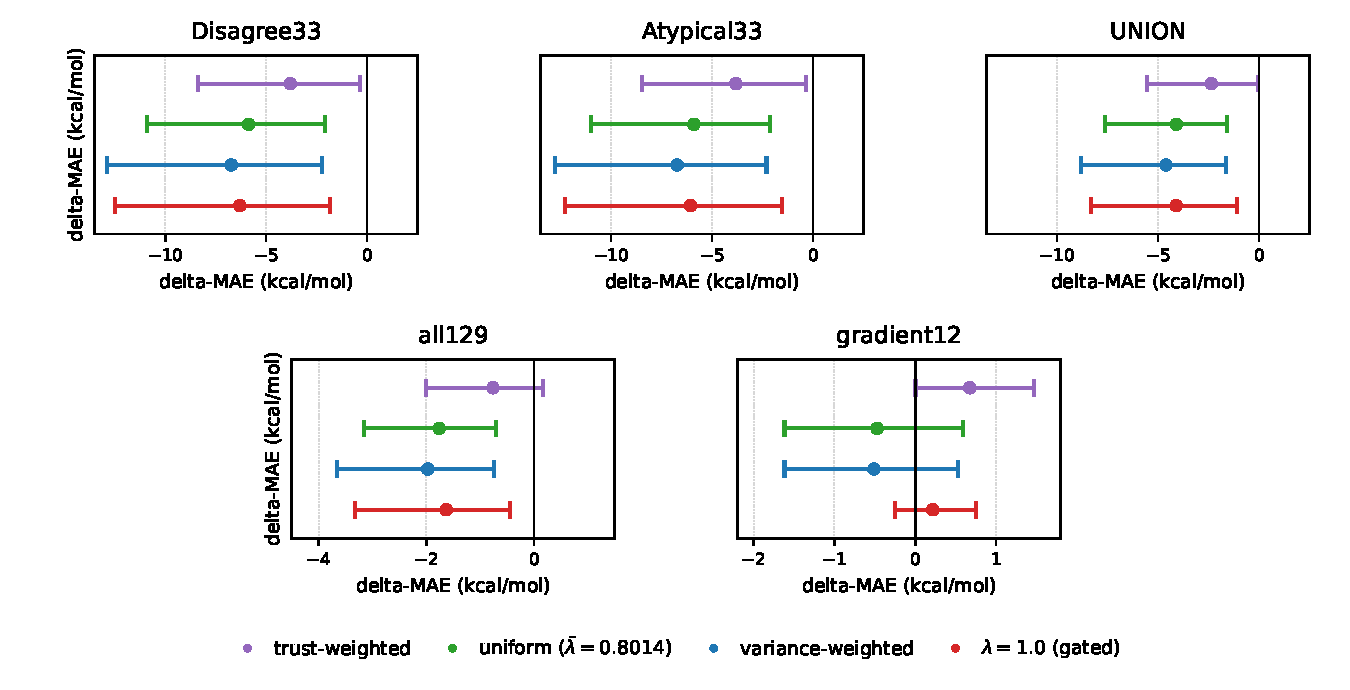
\includegraphics[width=0.88\textwidth]{fig_arms_forest.pdf}
  \caption{Forest plot of the four correction methods of
  Table~\ref{tab:arms}. Per-method $\Delta$MAE (kcal/mol) against the
  uncorrected ensemble mean on the five fold-0 populations, with
  10{,}000 paired-bootstrap 95\% confidence intervals (vertical line at
  zero; negative values are improvements). Built directly from the archived
  method-level result records.}
  \label{fig:arms-forest}
\end{figure}


\section{Extended Shrinkage-target Search}
\label{app:shrinkage-search}

We tested six alternative atom-level shrinkage designs, all more elaborate
than the plain variance-weighted (VW) method, which uses a fixed target (the
global pool mean). Each was calibrated on the same 102-molecule validation
set, evaluated on the same five fold-0 test populations with the same
10{,}000-draw paired bootstrap, and re-checked on the H2 holdout. Through
the Gauge lens, all six are still atom-level corrections, so they are
structurally capped in the same way VW is.

(1) \emph{Variance-Moderated} shrinkage adds a per-atom cutoff $d_0$ to the
VW formula. Its calibrated optimum is $d_0=0$, so it collapses back to VW. \par
(2) \emph{Element-Conditional} shrinkage replaces the global target with
per-element pool means. It underperforms VW on both validation and test. \par
(3) \emph{Two-Stage within-Molecule} shrinkage adds a second correction
using molecule-level variance; at its calibrated optimum this second stage
does nothing, and any active use of it hurts validation performance. \par
(4)
\emph{Magnitude-Adaptive (James--Stein)} shrinkage lets large-deviation
atoms shrink less. Its validation optimum is the limit where it reduces
exactly to VW, consistent with large-deviation atoms being no more reliable
than the rest. \par
(5) \emph{Hierarchical Element-Conditional} shrinkage lets
per-element means themselves shrink toward the global mean. This is the
only design that beats VW on validation, but the improvement reverses sign
on test and does not survive H1 recalibration -- evidence of overfitting to
the small validation set. \par
(6) \emph{Correlation-Aware Joint Shrinkage} uses
a single calibrated scalar to regularize the full per-molecule covariance
between atoms. Despite real cross-atom correlation in the raw predictions
(median $|\text{corr}|=0.83$), its calibrated optimum reduces it exactly to
VW, and it underperforms VW on validation.

In summary, every alternative design either reduces back to VW at its
calibrated optimum or performs worse than it. The one design that appeared
to beat VW did not hold up out of sample. Full per-design results are in
the supplementary verification records.

\section{Gauge-Invariant Ablations}
\label{app:gims-ablations}

We test three follow-up GIMS variants to probe the limits of Gauge
invariance. All three are negative or supporting ablations and none change
the main headline result.

\paragraph{GIMS-Total} This variant uses only the variance of the observable
molecular total, $\Lambda_m^{\mathrm{total}} = \dfrac{\operatorname{Var}_k(E_m^{(k)})}
{\operatorname{Var}_k(E_m^{(k)})+\tau_E^2}$, with no atomic variances at
all. This makes it invariant to an even wider class of atomic reallocations
than GIMS. Performance is slightly worse (test all129: $-1.95$ vs.\ GIMS's
$-2.00$; H2: $-2.85$ vs.\ $-2.94$; differences not significant). GIMS-total
is a useful theoretical check, but GIMS remains our primary method, since
its atomic variances give it a molecule-level coefficient with more signal
in it.
% VERIFIED. GIMS-total -1.9456 vs GIMS -2.0038 test all129 and H2 -2.85 vs -2.94 = gims_report.json gims_total vs gims_train and Gauge_INVARIANT_SHRINKAGE_RESULTS.md; diff +0.06 and +0.09 as above.

\paragraph{GIMS/VW blend} We blend the two corrections,
$E_{\mathrm{blend}}=(1-\alpha)E_{\mathrm{GIMS}}+\alpha E_{\mathrm{VW}}$, with
$\alpha$ chosen on validation ($\alpha=0.75$) and re-selected on H1
($\alpha=0.80$), leaning toward VW. The blend is not significantly
different from either GIMS or VW alone, and its point estimate is worse
than GIMS's, so we treat this as a negative ablation.
% VERIFIED. blend alpha 0.75 val and 0.80 H1, blend vs VW -0.028 and -0.046, vs GIMS +0.052/+0.053 = node_refinement/Gauge_invariant_shrinkage/gims_vw_blend_report.json and gims_vw_blend_results.csv and Gauge_INVARIANT_SHRINKAGE_RESULTS.md Final Interpretation.

\paragraph{CAAT} Composition-Aware Affine Transfer extends the external-set
affine fix with per-element terms, $\tilde E_m = aE_m + b_0 + \sum_e b_e
N_e$, where $N_e$ counts atoms of element $e$. Because a zero-sum atomic
shift leaves every $N_e$ unchanged, CAAT respects the same Gauge as GIMS.
It beats a plain affine fit on all three external populations. But against
a size-matched control with the same flexibility but no element
information, the improvement is significant only on the two hardest
populations, not overall. The largest per-element coefficients (P, Br) are
also fit on the least data (8--17 molecules per fold), so it remains
unclear whether the gain reflects real element-specific chemistry or is
just concentrated on a few rare, hard molecules. We report CAAT as a
promising but not yet conclusive extension.
% VERIFIED. CAAT all620/top155/worst62 = node_refinement/composition_aware_affine/composition_aware_results.csv; size-only control and coefficient stability/support = node_refinement/caat_diagnostics/CAAT_DIAGNOSTICS_REPORT.md.

Full tables for the permutation control and the train-only vs.\ pooled
reconciliation are included in the supplementary verification records.
% VERIFIED. permutation and reconciliation tables = node_refinement/Gauge_invariant_shrinkage/gims_additional_checks.json and docs/progress/GIMS_ADDITIONAL_CHECKS_RESULTS.md.

\section{Bias--Variance decomposition of the shrinkage gain}
\label{app:bias-var}

The shrinkage gain decomposes exactly, per molecule, into a bias-squared
term and a variance term ($\mathrm{MSE}_m = b_m^2 + v_m$, exact to machine
precision for every method and molecule). This lets us explain the small gap
between VW and uniform from Section~\ref{sec:method}'s covariance identity,
\[
\hat{E}_{m,\mathrm{VW}}^{(k)} - \widetilde{E}_{m,\mathrm{GIMS}}^{(k)}
= -N_m \operatorname{Cov}_{i=1,\dots,N_m}(\lambda_{mi},P_{mi}^{(k)}) .
\]It comes from
variance, not bias.

On the four main populations, about two-thirds of every method's MSE reduction
comes from bias-squared (0.65--0.67 across methods), so the methods mainly differ
in the remaining third, the variance term. On all129, VW and the gated method
leave little residual variance ($v\approx0.3$--$0.7$ (kcal/mol)$^2$),
uniform leaves more (2.6), and trust-weighted refinement leaves the most
(6.1). Gradient-12 is the exception: bias-squared dominates so completely
that uniform and VW's variance actually increases slightly, and the two
gated methods increase MSE outright there. Table~\ref{tab:bias-var} gives the
full per-method, per-population breakdown. Note this decomposition is in MSE
space and is therefore distinct from the MAE-space numbers in
Table~\ref{tab:arms}.

\begin{table}[htbp]
  \caption{Bias--variance decomposition of the shrinkage gain, per method and
  population, in (kcal/mol)$^2$. $b^2$ and $v$ are the post-correction
  bias-squared and variance; $\Delta$MSE is the change in mean squared
  error (negative means improvement); the last column is the fraction of
  that improvement coming from bias-squared (left blank where MSE got
  worse). Populations are defined in Section~\ref{sec:setup}.}
  \label{tab:bias-var}
  \centering
  \renewcommand{\arraystretch}{1.30}
  \small
  \setlength{\tabcolsep}{11pt}
  \begin{tabular}{ll@{\hspace{6pt}}rrrrr}
    \toprule
    Method & Population & $n$ & $b^2$ & $v$ & $\Delta$MSE & $b^2$ frac \\
    \midrule
    Trust-weighted & disagree33 & 33 & 73.85 & 23.47 & $-408.73$ & 0.655 \\
    Trust-weighted & atypical33 & 33 & 80.01 & 23.32 & $-411.35$ & 0.659 \\
    Trust-weighted & union50 & 50 & 64.20 & 15.52 & $-269.64$ & 0.655 \\
    Trust-weighted & all129 & 129 & 32.86 & 6.10 & $-103.25$ & 0.650 \\
    Trust-weighted & gradient12 & 12 & 18.85 & 0.12 & $+2.90$ & -- \\
    \midrule
    Uniform (matched) & disagree33 & 33 & 38.16 & 8.18 & $-459.71$ & 0.660 \\
    Uniform (matched) & atypical33 & 33 & 45.07 & 7.82 & $-461.77$ & 0.663 \\
    Uniform (matched) & union50 & 50 & 37.58 & 5.55 & $-306.24$ & 0.664 \\
    Uniform (matched) & all129 & 129 & 19.86 & 2.61 & $-119.75$ & 0.669 \\
    Uniform (matched) & gradient12 & 12 & 10.18 & 0.67 & $-5.21$ & 1.089 \\
    \midrule
    Variance-weighted (VW) & disagree33 & 33 & 27.17 & 0.87 & $-478.01$ & 0.658 \\
    Variance-weighted (VW) & atypical33 & 33 & 34.00 & 0.55 & $-480.12$ & 0.661 \\
    Variance-weighted (VW) & union50 & 50 & 30.11 & 0.74 & $-318.51$ & 0.662 \\
    Variance-weighted (VW) & all129 & 129 & 16.68 & 0.73 & $-124.81$ & 0.668 \\
    Variance-weighted (VW) & gradient12 & 12 & 9.61 & 0.62 & $-5.83$ & 1.071 \\
    \midrule
    Gated (top-quartile) & disagree33 & 33 & 29.51 & 0.45 & $-476.09$ & 0.656 \\
    Gated (top-quartile) & atypical33 & 33 & 38.43 & 0.29 & $-475.96$ & 0.657 \\
    Gated (top-quartile) & union50 & 50 & 34.15 & 0.38 & $-314.83$ & 0.656 \\
    Gated (top-quartile) & all129 & 129 & 19.60 & 0.27 & $-122.35$ & 0.657 \\
    Gated (top-quartile) & gradient12 & 12 & 16.20 & 0.14 & $+0.28$ & -- \\
    \bottomrule
  \end{tabular}
\end{table}

\newpage

%%%%%%%%%%%%%%%%%%%%%%%%%%%%%%%%%%%%%%%%%%%%%%%%%%%%%%%%%%%%

\newpage
\input{checklist.tex}

\end{document}
